\section {Wstęp}
\subsection {Czym jest LIDAR ?}

Za wikipedią:
Lidar (od angielskiego akronimu LIDAR, utworzonego od wyrażenia: Light Detection and Ranging)
– urządzenie działające na podobnej zasadzie jak radar (Radio Detection and Ranging), ale
wykorzystujące światło lasera zamiast mikrofal. Urządzenie charakteryzuje się wysoką
rozdzielczością \cite{lidar_pl}.\\

Pierwsze użycie lasera do pomiaru odległości miało miejsce na potrzeby amerykańskiego 
wojska na początku lat 60, zaraz po wynalezieniu lasera. Było to użycie laserowego dalmierza 
model Colidar Mark II - obiekt, ze względu na swoje rozmiary, przypominał strzelbę \cite{lidar_en}.\\

Pierwsze zastosowanie urządzeń przypominających obecne Lidary to rok 1971 i działalność
Amerykańskiego Centrum Badań Fizyki Atmosfery w Boulder w Kolorado (National Center for
Atmospheric Research). Urządzenie dokonywało pomiaru wysokości chmur i zanieczyszczenia
atmosferycznego. Kolejne zastosowanie tego samego roku miało miejsce w czasie misji
Apollo 15 gdzie za pomocą sonaru laserowego (tak technologia ta była wówczas nazywana)
skanowano powierzchnię księżyca \cite{lidar_en}.\\

Ogólna zasada działania polega na połączeniu lasera z teleskopem. Laser wysyła, poprzez 
układ optyczny, bardzo krótkie i dokładnie wymierzone, ale silne impulsy elektromagnetyczne
w widmie światła widzialnego lub podczerwonego. Na przebytym dystansie światło to ulega
rozproszeniu, które jest obserwowane za pomacą teleskopu, fotodiody, fotopowielacza albo
kamer CCD lub CMOS. \\

Zasadę te doskonale ilustruje rysunek z książki Paula McManamoma:
Figure 1.2 LiDAR Conceptual diagram (adapted from Ref. 3) \cite{mcmanamom}.\\
\begin{figure}[h]
    \centering
    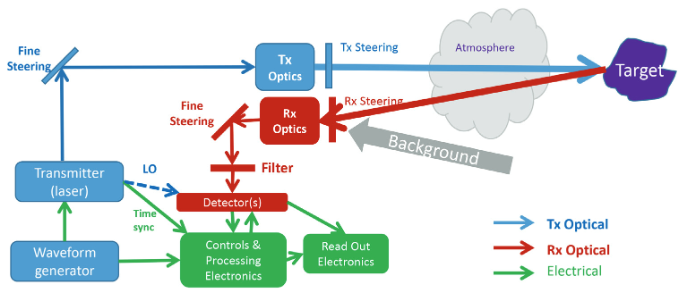
\includegraphics[scale=0.5]{lidar_concept}
    \caption{Rysunek z książki Paula McManamoma - LiDAR Conceptual diagram}
    \label{fig:lidar_concept}
\end{figure}

Dr. Pinliang Dong w swojej książce "LiDAR Remote Sensing and Applications" prezentuje 
wpływ zjawisk atmosferycznych na pomiary Lidaru \cite{dong}, jednak w mojej pracy pomiarów dokonywałem
jedynie w pomieszczeniach zamkniętych (co z resztą sugerowała specyfikacja dalmierza TFmini
Plus gdzie deklarowana przez producenta dokładność podana była dla pomieszczeń zamkniętych).\\

\subsection {Cel pracy}
Celem pracy jest zbudowanie działającej implementacji (zarówno sprzętowej jak i programowej) lidaru
dwuwymiarowego za pomocą dalmierza laserowego oraz silnika krokowego. Te dwa urządzenia będą
rdzeniem implementacji która za pośrednictwem mikrokontrolera będzie w stanie przekazać do komputera
dane z których napisany przez nas program wygeneruje dwuwymiarowy obraz pomieszczenia.